\documentclass{IOS-Book-Article}
\usepackage{mathptmx}
\usepackage{multirow}
\usepackage{graphicx}
\usepackage[utf8]{inputenc}
\usepackage[T1]{fontenc}
\usepackage[brazil]{babel}
% A classe do IOS traz rótulo de palavras-chave em inglês, alemão, francês e espanhol. Sem
% a versão em português o rótulo sai vazio e só o separador aparece, como um ponto solto.
% O `@` no nome exige \makeatletter: sem ele o LaTeX lê \keywordsname seguido de `@brazil`
% e reclama que o comando já existe.
\makeatletter
\newcommand{\keywordsname@brazil}{Palavras-chave}
\makeatother
\begin{document}
\begin{frontmatter}
\title{Medindo a competência de LLMs no direito brasileiro: responder, redigir e julgar}
\author[A]{\fnms{Eduardo} \snm{Pacheco}}
and
\author[A]{\fnms{Cibele Maria} \snm{Russo}}
\runningauthor{E. Pacheco e C. M. Russo}
\address[A]{Instituto de Ciências Matemáticas e de Computação, Universidade de São Paulo}
\begin{abstract}
Avaliar respostas jurídicas abertas em escala depende de usar um modelo de linguagem como corretor, e escolher qual modelo será o corretor é feito medindo a concordância dele com anotação humana e ordenando os candidatos numa tabela. Medimos 31 modelos nos três papéis que esse arranjo envolve, sobre as mesmas 105 questões da segunda fase do Exame de Ordem e os mesmos 940 critérios do espelho oficial, com padrão-ouro de 3 juristas: como respondentes na questão discursiva, como respondentes na redação de peça e como juízes das respostas alheias. As três ordens são reportadas por área do direito. São 3 resultados. Julgar e responder são competências associadas, mas a associação enfraquece conforme a tarefa deixa de cobrar forma e passa a cobrar mérito: $\rho$ = 0,67 na questão discursiva, 0,61 nos critérios formais da peça e 0,41 nos de mérito. A peça não é uma tarefa só: separada nas duas classes de critério que a própria banca rotula, a concordância do juiz é maior na parte formal do que na de mérito em 25 dos 26 juízes medidos, com diferença mediana de 0,168, as duas ordens concordam apenas a $\rho$ = 0,48, e o primeiro colocado não é o mesmo. E o número único por juiz esconde mais do que mostra: entre os nove primeiros colocados, que o piso de ruído do protocolo empata num vão de 0,047, a concordância de um mesmo juiz varia entre áreas do direito com mediana de 0,279, quase 6 vezes esse vão. Essa variação, porém, tem o tamanho da incerteza amostral por área: escolher um juiz por área não compensa fora da amostra, enquanto o voto majoritário dos cinco melhores juízes eleva o $\kappa$ em cerca de 0,04 em todas as tarefas.
\end{abstract}
\begin{keyword}
Benchmark \sep LLM-as-a-Judge \sep Brazil \sep Law \sep Reproducibility
\end{keyword}
\end{frontmatter}

\section{Introdução}

Avaliar se um modelo de linguagem respondeu bem a uma questão jurídica aberta é caro. Não há chave de resposta única, e comparação de cadeias de caracteres não funciona, porque duas respostas corretas podem não ter uma palavra em comum. A alternativa humana, contratar juristas para ler cada resposta, não escala para dezenas de modelos em centenas de questões. A saída adotada pela área é usar um modelo de linguagem como corretor, a técnica conhecida como \emph{LLM-as-judge} [1]. Dá-se ao corretor a resposta avaliada e os critérios de correção, e pede-se um veredito para cada um. Isso viabiliza a escala, mas empurra o problema um passo para trás: como saber se o corretor corrige bem? A resposta padrão é calibrá-lo contra anotação humana. Juristas anotam uma amostra, mede-se a concordância entre cada modelo candidato e essa anotação, e escolhe-se o que concorda mais. A concordância é medida pelo $\kappa$ de Cohen [7], que é a proporção de acertos descontada da concordância esperada por acaso. O desconto importa: se 80\% dos critérios têm resposta "não cumpriu", um juiz que responda sempre "não cumpriu" acerta 80\% sem saber nada, e o $\kappa$ dele é zero. Na convenção da área, $\kappa$ acima de 0,80 é considerado concordância forte. Esse arranjo põe os modelos em três papéis distintos sobre o mesmo material: escrever uma peça processual, responder uma questão discursiva e julgar o que os outros escreveram. A prática corrente trata os três como se fossem uma competência só, e é o que autoriza escolher o juiz pelo desempenho dele na tarefa, sem anotação humana. Este trabalho mede os mesmos 31 modelos nos três papéis, sobre o mesmo conjunto de questões e o mesmo espelho de correção, e reporta cada papel por área do direito. Os três resultados que se seguem são consequências dessa medição conjunta, e nenhum deles aparece numa tabela agregada de um número por modelo. Os vereditos dos 31 candidatos sobre os 940 critérios, em até 5 repetições cada, e as anotações dos três juristas que formam o padrão-ouro estão depositados em \texttt{10.5281/zenodo.22739161} [11], com soma de verificação por arquivo. O corpus de treino e os julgamentos das 180 condições do estudo companheiro [10] estão em \texttt{10.5281/zenodo.22739216} [12] e \texttt{10.5281/zenodo.22739184} [13], e o código em [14].

\section{Trabalhos relacionados}

O uso de modelos como avaliadores foi sistematizado por Zheng et al. [1], que também documentaram vieses do procedimento, de posição, de verbosidade e de auto-preferência. Trabalhos posteriores mostraram que os modelos reconhecem e favorecem as próprias gerações [18], que uma porcentagem alta de concordância com humanos pode esconder uma concordância baixa depois de descontado o acaso, e ordens que mudam com a métrica [15], que os juízes falham em pares construídos para separar o cumprimento da instrução da qualidade superficial [17], e que juízes fortes ficam perto do acaso em comparações difíceis e objetivamente verificáveis [16]. A forma de reporte, porém, permaneceu a mesma: uma tabela de concordância, ordenada, com um número por juiz. A concordância descontada do acaso tem limites próprios conhecidos: o $\kappa$ depende da prevalência da classe positiva e pode ser baixo quando a concordância bruta é alta [19], o que motiva alternativas ajustadas à prevalência, como o PABAK [20] e o AC1 de Gwet [21]. Em avaliação jurídica, o LegalBench [2] evita o problema usando tarefas de resposta curta e verificável, ao custo de se afastar da prática profissional.

Para o português jurídico há 3 conjuntos de avaliação diretamente relevantes, todos construídos sobre exames reais, e dois deles sobre o mesmo que usamos. O oab-bench [3] toma 105 questões de sete áreas do direito em edições recentes do Exame de Ordem e as corrige numa escala 0--10 contra o espelho da banca, reportando correlação forte entre as notas de um modelo de fronteira e as humanas. O Magis-Bench [4] passa ao judiciário, com 74 questões de oito concursos para a magistratura entre 2023 e 2025, cobrindo análise discursiva e redação de sentenças cível e criminal, corrigidas por quatro modelos de fronteira atuando como juízes. O Rabula [5] é construído sobre o Exame de Ordem de 2024 com quatro tarefas, corrige as generativas contra os critérios da própria banca como perguntas binárias ponderadas por dificuldade, e calibra o juiz automático pela concordância de Cohen com 3 juristas. Deste último herdamos o conjunto de avaliação, o padrão-ouro humano e o procedimento de correção, sem modificá-los.

Esses benchmarks reportam o desempenho dos respondentes por tarefa e, em parte, por área do direito, e o Rabula reporta a concordância do juiz como um número por candidato. Nenhum deles separa a redação de peça nas classes de critério que a banca rotula, nem reporta a concordância do juiz por área do direito, nem mede os mesmos modelos como respondentes e como juízes para comparar as duas ordens. A nossa contribuição é essa medição conjunta, decomposta por área e por classe de critério, acompanhada de um piso de ruído medido para a concordância do juiz. Sobre a reprodutibilidade da inferência, é conhecido que a não associatividade da aritmética de ponto flutuante torna o resultado dependente do agrupamento das operações [6]; o que não encontramos na literatura de \emph{LLM-as-judge} é o reconhecimento de que isso faz da configuração do servidor, tamanho de lote incluído, um parâmetro do protocolo, ao lado da temperatura e da semente.

\section{Materiais e métodos}

\subsection{As duas tarefas e o que cada uma cobra}

O conjunto de avaliação é composto por 105 questões da segunda fase do Exame de Ordem, provenientes dos exames 39, 40 e 41, com 35 de cada. Elas cobrem sete áreas do direito com exatamente 15 questões cada, de modo que nenhuma área domina a média. São 84 questões discursivas e 21 casos práticos que pedem a redação de uma peça processual, e os dois gêneros cobram coisas diferentes.

A questão discursiva apresenta um caso curto, mediana de 182 palavras, e faz de duas a quatro perguntas objetivas de direito sobre ele. Um caso de direito administrativo do exame 41 descreve uma desapropriação de imóvel rural pela União e pergunta se o poder público deve apresentar oferta de indenização antes de ajuizar a ação e se cabe arbitragem no procedimento. A resposta esperada é curta e o espelho a decompõe em poucos critérios, mediana de 4 e no máximo 7: um exige a tese correta, "o poder público deverá notificar o proprietário e apresentar oferta de indenização antes do ajuizamento", valendo 0,5 ponto, e outro exige a fundamentação, "nos termos do Art. 10-A do Decreto-Lei n\textsuperscript{o} 3.365/1941", valendo 0,1. O que se cobra é conteúdo jurídico, sem exigência de forma documental.

A redação de peça apresenta um caso mais longo, mediana de 399 palavras, e pede uma peça processual completa na posição de advogado de uma das partes. O espelho decompõe a peça em muito mais critérios, mediana de 26 e até 38, e eles vêm rotulados por título. Num mandado de segurança contra ato de presidente de comissão de licitação, os primeiros critérios são "Endereçamento: a peça deve ser endereçada ao Juízo da Vara Cível ou da Vara de Fazenda Pública da Comarca", "Qualificação das partes: autoridade coatora, João da Silva, presidente da Comissão de Licitação" e "Cabimento: houve violação a direito líquido e certo". Além do conteúdo jurídico, cobra-se o esqueleto do documento.

\begin{table}[!ht]
\centering
\caption{Composição do conjunto de avaliação e do padrão-ouro humano. A unidade de análise não é a questão e sim o critério, uma afirmação binária sobre a resposta extraída do espelho oficial.}
\footnotesize\setlength{\tabcolsep}{2pt}
\begin{tabular}{llrrrr}
\hline
\textbf{Gênero} & \textbf{Questões} & \textbf{Critérios} & \textbf{de forma} & \textbf{de mérito} & \textbf{$\kappa$ entre humanos} \\
\hline
Questão discursiva & 84 & 379 & -- & 379 & 0,789 \\
Redação de peça & 21 & 561 & 148 & 413 & 0,763 \\
\hline
\end{tabular}
\par\vspace{3pt}\begin{minipage}{\textwidth}\footnotesize A concordância entre os três anotadores humanos é medida com $\kappa$ de Fleiss [8]. Ela estabelece o teto realista de qualquer juiz automático: um juiz que marque 0,824 em discursiva concorda com o consenso humano mais do que os humanos concordam entre si.\end{minipage}
\end{table}


\subsection{As duas classes de critério na peça}

Os títulos com que a banca rotula os critérios da peça se dividem em duas famílias. Os de forma cobrem o esqueleto do documento: endereçamento ao juízo competente, qualificação das partes, tempestividade, requisitos de admissibilidade, fechamento com local, data e assinatura. Os de mérito cobrem a tese jurídica, os fundamentos e os pedidos. São 148 e 413, respectivamente, e todos os critérios formais estão em peças, porque questões discursivas não têm esqueleto de documento a cumprir. O agrupamento dos títulos nas duas famílias é nosso; os títulos, não. A separação importa porque as duas classes pedem operações cognitivas diferentes, tanto de quem escreve quanto de quem corrige. Decidir se a peça foi endereçada ao juízo competente é aproximar um trecho de texto de um gabarito curto. Decidir se houve violação a direito líquido e certo é avaliar uma tese. Não há razão para supor que um mesmo modelo seja igualmente bom nas duas, e a Seção 4.3 mostra que não é.

\subsection{Os três papéis e o protocolo de medição}

Cada um dos 31 modelos foi medido nos três papéis. Como respondente, recebe o enunciado e produz a resposta ou a peça, com temperatura 0,7, teto de 2.500 tokens de saída e três execuções por questão. As respostas são corrigidas pelos dois juízes escolhidos por este protocolo, o Kimi K2.5 na questão discursiva e o GPT-OSS 120B na peça, com o mesmo procedimento de julgamento descrito abaixo, e a nota é o percentual dos pontos da banca, ponderado pela pontuação de cada critério. Esses dois juízes também são respondentes e corrigem as próprias respostas, um risco de auto-preferência [1] que reportamos e não corrigimos. Como juiz, recebe a resposta de outro modelo, o espelho da banca e a lista completa de critérios daquela questão, sem o enunciado do caso, e devolve numa única resposta estruturada em JSON um veredito binário para cada critério. Os vereditos são comparados ao padrão-ouro de 940 decisões tomadas por 3 juristas experientes sobre respostas escritas pelo GPT-4o mini, ambos herdados do Rabula [5]. O Apêndice A traz o prompt de julgamento, o Apêndice B um item completo com os vereditos humanos e automáticos, o Apêndice C a configuração de cada juiz e o Apêndice D o agrupamento dos títulos de critério em classes. A concordância é medida por $\kappa$ de Cohen, separadamente por gênero, por classe de critério e por área do direito.

O protocolo inteiro foi repetido até 5 vezes por candidato. Os juízes rodam a temperatura 0,2 e sem semente, que a API Converse do Amazon Bedrock, por onde passam 29 dos 31 juízes, não aceita, e cada repetição é um voto de maioria sobre três amostras; os cinco modelos Claude, repescados sob cota menor, têm uma única amostra, e onde só duas amostras são válidas o empate conta como cumprido. O teto de saída depende do modelo: 2.048 tokens para o Llama 3 e os Mistral menores, 16.000 para os modelos de raciocínio e 8.000 para os demais, dobrado quando a resposta é cortada. O modelo de prompt não mudou entre as repetições, mas toda chamada leva um token aleatório e pede a soma de dois inteiros aleatórios, um quebra-cache herdado do Rabula que impede o provedor de devolver uma resposta guardada. O código de julgamento recebeu correções de nova tentativa e de teto de saída ao longo das rodadas, nenhuma tocando o prompt. As repetições medem, portanto, a dispersão do $\kappa$ sob amostragem, que é a variação que enfrenta quem usa o mesmo juiz, e dela deriva o limiar de decisão usado adiante. A cobertura não é uniforme entre candidatos: 26 juízes completaram as 5 repetições, três completaram três por cota de API, e dois não produziram resultado utilizável em peça. Um juiz só é pontuado se cobrir ao menos 85\% dos critérios do gênero, e se o que falta faltar por acaso, o que se verifica por teste exato de Fisher sobre a tabela de julgado contra omitido por resposta humana positiva contra negativa.

\section{Resultados}

As Tabelas 2 e 3 trazem a concordância de cada juiz com o padrão-ouro humano, por área do direito, uma por gênero, com a peça separada nas duas classes de critério. As Tabelas 4 e 5 trazem, no mesmo desenho, a nota dos mesmos modelos como respondentes. As tabelas mostram os 22 juízes de melhor concordância em mérito de peça, que é o que cabe na página; os 26 que produziram resultado nas três tarefas estão no depósito [11], com a mesma decomposição. Toda estatística reportada adiante é calculada sobre os 26, e não sobre o recorte exibido, que é selecionado por uma das variáveis em questão.

\begin{table}[!ht]
\centering
\caption{Concordância de Cohen com o padrão-ouro humano na \textbf{questão discursiva}, por área do direito. Valores $\times$100. A coluna \textbf{ampl.} é a distância entre a melhor e a pior área do mesmo juiz.}
\footnotesize\setlength{\tabcolsep}{2pt}
\begin{tabular}{llrrrrrrrr}
\hline
\textbf{Juiz} & \textbf{Adm.} & \textbf{Civ.} & \textbf{Const.} & \textbf{Empr.} & \textbf{Pen.} & \textbf{Trab.} & \textbf{Trib.} & \textbf{geral} & \textbf{ampl.} \\
\hline
\texttt{claude-opus-4-6} & 78 & 74 & 92 & 74 & 88 & 73 & 82 & 80 & 18 \\
\texttt{gpt-oss-120b} & 72 & 78 & 89 & 78 & 85 & 76 & 93 & 82 & 21 \\
\texttt{claude-opus-4-5} & 82 & 81 & 91 & 78 & 84 & 77 & 82 & 82 & 13 \\
\texttt{kimi-k2-5} & 83 & 83 & 81 & 78 & 70 & 74 & 88 & 80 & 18 \\
\texttt{kimi-k2-thinking} & 80 & 81 & 85 & 77 & 81 & 76 & 85 & 81 & 9 \\
\texttt{glm-4-7} & 71 & 85 & 86 & 85 & 77 & 81 & 86 & 82 & 15 \\
\texttt{claude-sonnet-4-5} & 63 & 88 & 86 & 73 & 87 & 81 & 75 & 81 & 25 \\
\texttt{sabia-4} & 72 & 84 & 92 & 79 & 81 & 77 & 88 & 82 & 19 \\
\texttt{claude-sonnet-4-6} & 64 & 77 & 96 & 73 & 79 & 77 & 69 & 77 & 32 \\
\texttt{claude-haiku-4-5} & 65 & 79 & 74 & 81 & 82 & 75 & 80 & 77 & 17 \\
\texttt{deepseek-v3} & 63 & 81 & 82 & 77 & 79 & 82 & 74 & 78 & 20 \\
\texttt{glm-5} & 66 & 85 & 87 & 78 & 71 & 87 & 80 & 80 & 21 \\
\texttt{minimax-m2-5} & 78 & 74 & 85 & 83 & 77 & 85 & 89 & 81 & 15 \\
\texttt{qwen3-235b-vl} & 71 & 84 & 78 & 88 & 69 & 74 & 79 & 78 & 19 \\
\texttt{mistral-l3-675b} & 62 & 82 & 79 & 83 & 70 & 81 & 83 & 77 & 21 \\
\texttt{mistral-large} & 82 & 80 & 83 & 84 & 70 & 67 & 83 & 79 & 17 \\
\texttt{magistral-small} & 68 & 80 & 67 & 79 & 45 & 69 & 86 & 70 & 41 \\
\texttt{nemotron-s3-120b} & 70 & 69 & 59 & 88 & 46 & 46 & 67 & 63 & 43 \\
\texttt{sabiazinho-4} & 70 & 77 & 88 & 82 & 67 & 71 & 82 & 76 & 22 \\
\texttt{qwen3-80b-a3b} & 64 & 82 & 80 & 78 & 42 & 69 & 86 & 71 & 44 \\
\texttt{llama4-maverick} & 84 & 79 & 86 & 84 & 59 & 77 & 84 & 79 & 27 \\
\texttt{qwen3-32b} & 74 & 76 & 62 & 80 & 61 & 67 & 78 & 71 & 20 \\
\hline
\end{tabular}
\end{table}


\begin{table}[!ht]
\centering
\caption{Concordância de Cohen com o padrão-ouro humano na \textbf{redação de peça}, por área do direito. Cada célula traz dois valores, \textbf{formal} | mérito, nas duas classes de critério que a banca rotula. Valores $\times$100. A coluna \textbf{ampl.} é a distância entre a melhor e a pior área do mesmo juiz.}
\footnotesize\setlength{\tabcolsep}{2pt}
\begin{tabular}{llrrrrrrrr}
\hline
\textbf{Juiz} & \textbf{Adm.} & \textbf{Civ.} & \textbf{Const.} & \textbf{Empr.} & \textbf{Pen.} & \textbf{Trab.} & \textbf{Trib.} & \textbf{geral} & \textbf{ampl.} \\
\hline
\texttt{claude-opus-4-6} & \textbf{89}|76 & \textbf{64}|69 & \textbf{91}|76 & \textbf{75}|57 & \textbf{65}|80 & \textbf{78}|73 & \textbf{91}|87 & \textbf{80}|74 & \textbf{27}|30 \\
\texttt{gpt-oss-120b} & \textbf{84}|73 & \textbf{78}|74 & \textbf{72}|57 & \textbf{75}|67 & \textbf{65}|73 & \textbf{77}|76 & \textbf{88}|85 & \textbf{78}|73 & \textbf{23}|28 \\
\texttt{claude-opus-4-5} & \textbf{91}|66 & \textbf{78}|65 & \textbf{91}|76 & \textbf{87}|62 & \textbf{75}|84 & \textbf{80}|67 & \textbf{88}|87 & \textbf{85}|73 & \textbf{16}|25 \\
\texttt{kimi-k2-5} & \textbf{80}|59 & \textbf{78}|77 & \textbf{74}|60 & \textbf{64}|66 & \textbf{69}|81 & \textbf{79}|61 & \textbf{88}|90 & \textbf{77}|72 & \textbf{24}|31 \\
\texttt{kimi-k2-thinking} & \textbf{82}|63 & \textbf{57}|74 & \textbf{72}|59 & \textbf{68}|65 & \textbf{67}|73 & \textbf{86}|61 & \textbf{93}|93 & \textbf{77}|71 & \textbf{36}|34 \\
\texttt{glm-4-7} & \textbf{87}|63 & \textbf{78}|69 & \textbf{82}|53 & \textbf{73}|63 & \textbf{75}|84 & \textbf{78}|71 & \textbf{88}|86 & \textbf{81}|70 & \textbf{15}|33 \\
\texttt{claude-sonnet-4-5} & \textbf{98}|61 & \textbf{78}|72 & \textbf{91}|62 & \textbf{87}|60 & \textbf{65}|79 & \textbf{79}|60 & \textbf{88}|86 & \textbf{84}|70 & \textbf{33}|26 \\
\texttt{sabia-4} & \textbf{82}|68 & \textbf{66}|67 & \textbf{84}|59 & \textbf{87}|62 & \textbf{85}|80 & \textbf{79}|60 & \textbf{88}|85 & \textbf{82}|70 & \textbf{22}|26 \\
\texttt{claude-sonnet-4-6} & \textbf{85}|57 & \textbf{78}|72 & \textbf{91}|71 & \textbf{75}|60 & \textbf{75}|83 & \textbf{80}|56 & \textbf{88}|79 & \textbf{83}|70 & \textbf{16}|27 \\
\texttt{claude-haiku-4-5} & \textbf{85}|52 & \textbf{76}|70 & \textbf{74}|53 & \textbf{68}|69 & \textbf{87}|73 & \textbf{78}|57 & \textbf{88}|85 & \textbf{80}|66 & \textbf{20}|33 \\
\texttt{deepseek-v3} & \textbf{91}|55 & \textbf{78}|63 & \textbf{77}|49 & \textbf{87}|63 & \textbf{75}|78 & \textbf{81}|58 & \textbf{88}|85 & \textbf{83}|65 & \textbf{16}|36 \\
\texttt{glm-5} & \textbf{91}|59 & \textbf{78}|53 & \textbf{82}|51 & \textbf{82}|68 & \textbf{73}|79 & \textbf{83}|62 & \textbf{88}|84 & \textbf{83}|65 & \textbf{18}|32 \\
\texttt{minimax-m2-5} & \textbf{75}|57 & \textbf{63}|64 & \textbf{79}|43 & \textbf{73}|58 & \textbf{73}|79 & \textbf{92}|59 & \textbf{88}|79 & \textbf{79}|63 & \textbf{29}|35 \\
\texttt{qwen3-235b-vl} & \textbf{91}|48 & \textbf{73}|59 & \textbf{72}|42 & \textbf{87}|62 & \textbf{75}|70 & \textbf{80}|65 & \textbf{88}|78 & \textbf{81}|61 & \textbf{19}|36 \\
\texttt{mistral-l3-675b} & \textbf{89}|54 & \textbf{71}|53 & \textbf{83}|42 & \textbf{79}|55 & \textbf{87}|75 & \textbf{86}|64 & \textbf{88}|81 & \textbf{84}|61 & \textbf{18}|39 \\
\texttt{mistral-large} & \textbf{81}|44 & \textbf{66}|66 & \textbf{63}|43 & \textbf{59}|59 & \textbf{75}|64 & \textbf{86}|66 & \textbf{88}|76 & \textbf{76}|61 & \textbf{29}|33 \\
\texttt{magistral-small} & \textbf{76}|45 & \textbf{82}|50 & \textbf{72}|35 & \textbf{62}|59 & \textbf{79}|72 & \textbf{87}|64 & \textbf{88}|64 & \textbf{80}|56 & \textbf{26}|37 \\
\texttt{nemotron-s3-120b} & \textbf{65}|46 & \textbf{76}|54 & \textbf{77}|31 & \textbf{61}|61 & \textbf{71}|60 & \textbf{87}|58 & \textbf{75}|72 & \textbf{75}|55 & \textbf{25}|41 \\
\texttt{sabiazinho-4} & \textbf{35}|59 & \textbf{37}|40 & \textbf{37}|54 & \textbf{36}|32 & \textbf{63}|74 & \textbf{63}|39 & \textbf{57}|71 & \textbf{51}|54 & \textbf{28}|42 \\
\texttt{qwen3-80b-a3b} & \textbf{64}|36 & \textbf{58}|48 & \textbf{62}|35 & \textbf{57}|59 & \textbf{65}|53 & \textbf{79}|57 & \textbf{88}|68 & \textbf{69}|51 & \textbf{31}|34 \\
\texttt{llama4-maverick} & \textbf{64}|54 & \textbf{88}|43 & \textbf{68}|28 & \textbf{87}|54 & \textbf{78}|49 & \textbf{89}|56 & \textbf{88}|66 & \textbf{81}|50 & \textbf{26}|38 \\
\texttt{qwen3-32b} & \textbf{73}|46 & \textbf{61}|35 & \textbf{56}|38 & \textbf{83}|51 & \textbf{84}|56 & \textbf{86}|59 & \textbf{88}|58 & \textbf{77}|49 & \textbf{32}|24 \\
\hline
\end{tabular}
\end{table}


\begin{table}[!ht]
\centering
\caption{Nota dos mesmos modelos como \textbf{respondentes} na questão discursiva, por área do direito.}
\footnotesize\setlength{\tabcolsep}{2pt}
\begin{tabular}{llrrrrrrr}
\hline
\textbf{Modelo} & \textbf{Adm.} & \textbf{Civ.} & \textbf{Const.} & \textbf{Empr.} & \textbf{Pen.} & \textbf{Trab.} & \textbf{Trib.} & \textbf{geral} \\
\hline
\texttt{claude-opus-4-6} & 94,9 & 91,2 & 89,6 & 85,2 & 87,5 & 93,5 & 79,2 & 88,8 \\
\texttt{gpt-oss-120b} & 55,1 & 60,9 & 40,9 & 42,9 & 53,7 & 50,6 & 41,3 & 49,3 \\
\texttt{claude-opus-4-5} & 93,8 & 87,4 & 87,3 & 87,8 & 85,7 & 95,2 & 83,2 & 88,6 \\
\texttt{kimi-k2-5} & 64,3 & 61,9 & 58,7 & 43,1 & 63,6 & 61,7 & 47,4 & 57,2 \\
\texttt{kimi-k2-thinking} & 53,9 & 47,7 & 54,6 & 52,6 & 48,4 & 50,9 & 42,4 & 50,6 \\
\texttt{glm-4-7} & 60,0 & 67,7 & 69,4 & 47,7 & 70,2 & 66,7 & 56,5 & 62,6 \\
\texttt{claude-sonnet-4-5} & 77,9 & 85,9 & 80,7 & 54,8 & 77,1 & 80,7 & 64,9 & 74,6 \\
\texttt{sabia-4} & 72,3 & 80,7 & 70,2 & 64,9 & 85,8 & 91,1 & 74,0 & 77,0 \\
\texttt{claude-sonnet-4-6} & 90,0 & 82,3 & 84,9 & 73,9 & 81,7 & 85,8 & 84,4 & 83,3 \\
\texttt{claude-haiku-4-5} & 60,0 & 65,4 & 54,1 & 50,8 & 57,1 & 48,9 & 46,6 & 54,7 \\
\texttt{deepseek-v3} & 73,1 & 64,3 & 68,0 & 55,1 & 69,2 & 49,6 & 45,7 & 60,7 \\
\texttt{glm-5} & 63,5 & 69,8 & 64,7 & 42,6 & 71,1 & 62,4 & 61,7 & 62,3 \\
\texttt{minimax-m2-5} & 62,3 & 73,2 & 71,7 & 49,4 & 70,4 & 57,8 & 57,8 & 63,0 \\
\texttt{qwen3-235b-vl} & 60,4 & 64,4 & 58,7 & 53,7 & 61,4 & 56,8 & 36,2 & 56,0 \\
\texttt{mistral-l3-675b} & 68,8 & 79,0 & 66,8 & 66,6 & 77,3 & 78,7 & 61,4 & 71,2 \\
\texttt{mistral-large} & 38,6 & 28,9 & 18,4 & 47,3 & 43,4 & 32,4 & 26,5 & 33,7 \\
\texttt{magistral-small} & 48,1 & 51,8 & 46,9 & 44,5 & 60,2 & 47,7 & 39,8 & 48,4 \\
\texttt{nemotron-s3-120b} & 53,8 & 53,5 & 46,7 & 47,6 & 53,9 & 49,3 & 46,6 & 50,2 \\
\texttt{sabiazinho-4} & 56,3 & 78,7 & 71,7 & 61,1 & 76,1 & 81,1 & 62,0 & 69,6 \\
\texttt{qwen3-80b-a3b} & 55,5 & 54,8 & 53,9 & 48,2 & 57,8 & 48,5 & 52,1 & 53,0 \\
\texttt{llama4-maverick} & 54,9 & 62,6 & 69,2 & 44,1 & 65,2 & 59,4 & 54,3 & 58,5 \\
\texttt{qwen3-32b} & 38,1 & 38,9 & 28,8 & 34,7 & 44,4 & 29,2 & 31,2 & 35,1 \\
\hline
\end{tabular}
\end{table}


\begin{table}[!ht]
\centering
\caption{Nota dos mesmos modelos como \textbf{respondentes} na redação de peça, em percentual dos pontos da banca. Mesma leitura das células: \textbf{formal} | mérito.}
\footnotesize\setlength{\tabcolsep}{2pt}
\begin{tabular}{llrrrrrrr}
\hline
\textbf{Modelo} & \textbf{Adm.} & \textbf{Civ.} & \textbf{Const.} & \textbf{Empr.} & \textbf{Pen.} & \textbf{Trab.} & \textbf{Trib.} & \textbf{geral} \\
\hline
\texttt{claude-opus-4-6} & \textbf{68,5}|32,7 & \textbf{40,1}|66,7 & \textbf{68,8}|66,4 & \textbf{43,8}|59,6 & \textbf{50,0}|63,8 & \textbf{53,6}|55,5 & \textbf{70,8}|68,4 & \textbf{55,5}|63,4 \\
\texttt{gpt-oss-120b} & \textbf{53,1}|29,6 & \textbf{59,0}|55,8 & \textbf{48,4}|50,6 & \textbf{50,7}|50,5 & \textbf{18,5}|25,7 & \textbf{20,1}|54,7 & \textbf{48,0}|62,8 & \textbf{42,5}|47,1 \\
\texttt{claude-opus-4-5} & \textbf{68,5}|46,4 & \textbf{62,0}|65,0 & \textbf{63,1}|60,4 & \textbf{61,3}|48,1 & \textbf{51,9}|55,4 & \textbf{46,0}|70,3 & \textbf{57,8}|65,5 & \textbf{58,6}|58,7 \\
\texttt{kimi-k2-5} & \textbf{38,3}|19,7 & \textbf{40,6}|45,0 & \textbf{39,8}|38,9 & \textbf{47,4}|30,5 & \textbf{13,0}|27,0 & \textbf{13,8}|43,7 & \textbf{26,1}|44,3 & \textbf{31,3}|35,6 \\
\texttt{kimi-k2-thinking} & \textbf{29,0}|11,1 & \textbf{52,2}|15,4 & \textbf{45,9}|17,9 & \textbf{40,7}|8,2 & \textbf{0,0}|23,7 & \textbf{19,1}|13,9 & \textbf{27,4}|30,7 & \textbf{30,6}|15,8 \\
\texttt{glm-4-7} & \textbf{63,6}|57,1 & \textbf{82,1}|71,6 & \textbf{79,8}|75,2 & \textbf{69,1}|54,8 & \textbf{51,9}|59,0 & \textbf{53,1}|70,4 & \textbf{68,4}|70,1 & \textbf{66,9}|65,5 \\
\texttt{claude-sonnet-4-5} & \textbf{72,8}|26,9 & \textbf{61,2}|49,5 & \textbf{61,7}|50,7 & \textbf{52,4}|48,6 & \textbf{46,3}|41,9 & \textbf{39,9}|30,7 & \textbf{39,6}|62,0 & \textbf{53,4}|44,3 \\
\texttt{sabia-4} & \textbf{74,7}|26,6 & \textbf{54,7}|67,6 & \textbf{59,7}|54,6 & \textbf{61,3}|46,6 & \textbf{79,6}|53,6 & \textbf{43,2}|47,5 & \textbf{60,0}|53,3 & \textbf{61,9}|50,0 \\
\texttt{claude-sonnet-4-6} & \textbf{64,8}|39,6 & \textbf{52,8}|55,1 & \textbf{63,1}|58,8 & \textbf{65,0}|43,6 & \textbf{31,5}|51,9 & \textbf{30,3}|44,1 & \textbf{52,0}|58,7 & \textbf{51,4}|50,2 \\
\texttt{claude-haiku-4-5} & \textbf{35,2}|14,1 & \textbf{46,6}|53,1 & \textbf{47,5}|49,3 & \textbf{45,2}|29,2 & \textbf{3,7}|34,9 & \textbf{18,3}|30,7 & \textbf{46,2}|48,6 & \textbf{34,7}|37,1 \\
\texttt{deepseek-v3} & \textbf{38,9}|34,9 & \textbf{72,9}|62,8 & \textbf{57,4}|75,4 & \textbf{56,7}|59,1 & \textbf{33,3}|57,6 & \textbf{29,1}|55,4 & \textbf{57,3}|59,1 & \textbf{49,4}|57,8 \\
\texttt{glm-5} & \textbf{61,7}|48,5 & \textbf{82,5}|67,2 & \textbf{70,3}|67,8 & \textbf{73,7}|53,5 & \textbf{33,3}|71,0 & \textbf{37,4}|69,9 & \textbf{63,6}|62,0 & \textbf{60,4}|62,8 \\
\texttt{minimax-m2-5} & \textbf{54,3}|24,2 & \textbf{57,6}|48,4 & \textbf{57,4}|48,7 & \textbf{49,2}|41,1 & \textbf{38,9}|41,7 & \textbf{26,8}|44,8 & \textbf{44,6}|45,4 & \textbf{46,9}|42,0 \\
\texttt{qwen3-235b-vl} & \textbf{35,8}|34,7 & \textbf{76,9}|59,3 & \textbf{45,8}|64,2 & \textbf{65,4}|50,9 & \textbf{25,9}|45,1 & \textbf{33,9}|52,8 & \textbf{52,2}|54,7 & \textbf{48,0}|51,7 \\
\texttt{mistral-l3-675b} & \textbf{63,0}|58,1 & \textbf{78,4}|73,2 & \textbf{82,6}|77,7 & \textbf{78,0}|63,1 & \textbf{42,6}|70,9 & \textbf{48,3}|72,4 & \textbf{70,3}|70,1 & \textbf{66,2}|69,3 \\
\texttt{mistral-large} & \textbf{24,1}|19,0 & \textbf{47,5}|32,4 & \textbf{48,0}|30,6 & \textbf{47,4}|29,0 & \textbf{27,8}|28,3 & \textbf{18,7}|16,5 & \textbf{44,3}|36,7 & \textbf{36,8}|27,5 \\
\texttt{magistral-small} & \textbf{45,7}|32,4 & \textbf{62,0}|50,5 & \textbf{61,2}|43,8 & \textbf{61,2}|46,8 & \textbf{44,4}|38,8 & \textbf{35,9}|43,6 & \textbf{52,3}|58,0 & \textbf{51,8}|44,8 \\
\texttt{nemotron-s3-120b} & \textbf{24,7}|28,3 & \textbf{52,0}|49,7 & \textbf{44,3}|64,2 & \textbf{46,1}|41,1 & \textbf{13,0}|36,0 & \textbf{15,8}|47,2 & \textbf{36,1}|47,9 & \textbf{33,1}|44,9 \\
\texttt{sabiazinho-4} & \textbf{67,3}|39,9 & \textbf{50,1}|69,1 & \textbf{60,5}|71,6 & \textbf{59,1}|41,3 & \textbf{51,9}|42,8 & \textbf{50,2}|48,1 & \textbf{63,3}|68,1 & \textbf{57,5}|54,4 \\
\texttt{qwen3-80b-a3b} & \textbf{33,3}|47,0 & \textbf{62,1}|61,3 & \textbf{43,9}|64,1 & \textbf{62,2}|45,4 & \textbf{24,1}|39,6 & \textbf{26,6}|54,3 & \textbf{37,4}|47,9 & \textbf{41,4}|51,4 \\
\texttt{llama4-maverick} & \textbf{49,4}|23,2 & \textbf{52,1}|39,3 & \textbf{62,1}|64,4 & \textbf{56,0}|43,6 & \textbf{40,7}|50,9 & \textbf{36,5}|43,1 & \textbf{68,8}|56,8 & \textbf{52,2}|45,9 \\
\texttt{qwen3-32b} & \textbf{35,2}|20,9 & \textbf{67,7}|38,9 & \textbf{47,0}|41,8 & \textbf{43,2}|38,2 & \textbf{25,9}|32,5 & \textbf{27,1}|41,7 & \textbf{48,2}|51,0 & \textbf{42,0}|37,9 \\
\hline
\end{tabular}
\end{table}


\subsection{A leitura direta das tabelas}

Três leituras saltam das colunas. A primeira é que o primeiro colocado depende da tarefa. Na questão discursiva e nos critérios formais da peça, o melhor juiz é o \texttt{claude-opus-4-5}, com 0,824 e 0,850; nos critérios de mérito, é o \texttt{claude-opus-4-6}, com 0,744. Nas notas, a dissociação é maior: o \texttt{claude-opus-4-6} tira 88,8\% dos pontos na discursiva e 55,5\% nos critérios formais da peça, e o \texttt{glm-4-7}, que tira 62,6\% na discursiva, chega a 66,9\% na parte formal da peça.

A segunda é que a variação entre áreas do direito é grande, e maior do que a variação entre juízes no topo. Entre os 26 medidos, a distância entre a melhor e a pior área do mesmo juiz tem mediana de 0,207 na discursiva, 0,256 nos critérios formais e 0,338 nos de mérito. A comparação que fecha o ponto é interna ao topo: os nove primeiros colocados em mérito de peça estão todos contidos num vão de 0,047, e a amplitude entre áreas dentro de um desses mesmos nove tem mediana de 0,279, quase seis vezes maior. Um juiz escolhido pela coluna agregada pode estar entre os melhores em direito tributário e entre os piores em penal, e a tabela de um número por juiz não registra isso.

A terceira é que a parte formal da peça é sistematicamente mais fácil de julgar do que a de mérito, e é a única das três fatias em que os melhores juízes alcançam o teto humano. A Seção 4.3 trata disso. Nem todo candidato chega às tabelas, e as ausências têm causas distintas que a célula vazia não separa. Julgar uma peça exige emitir veredito estruturado sobre até 38 critérios de uma vez, e modelos com teto de saída de 4.096 tokens não produzem essa resposta inteira: os dois Llama 3 cobrem 9\% e 19\% dos critérios de peça, e são ausência por limite estrutural. O Mixtral 8x7B cobre 91\%, ou seja, responde quase tudo, e ainda assim marca $\kappa$ de 0,123, concordância quase nula. O \texttt{sabiazinho-4} cobre 93\% e omite o resto, e o que ele omite não é aleatório quando a omissão é sistemática: os 63 critérios deixados de fora em três ou mais das 5 repetições têm 60,3\% de resposta humana positiva contra 38,0\% do restante (Fisher, p = 0,0010), ou seja, ele se cala preferencialmente sobre os critérios fáceis. Incapacidade estrutural, capacidade com concordância nula e omissão seletiva são três situações diferentes, e as três aparecem como falta de nota.

\subsection{O piso de ruído e o empate no topo}

Rodar o mesmo protocolo, com o mesmo prompt, sobre os mesmos dados, não devolve o mesmo número. O desvio típico mediano do $\kappa$ entre repetições é de 0,0101. No nível do veredito, a fração de critérios de peça cujo veredito muda entre as repetições de um juiz fica entre 2,9\% e 6,1\% entre os nove primeiros e chega a 18,4\% no menos estável. Convertido num limiar de decisão a 95\% de confiança, duas notas que diferem por menos de cerca de 0,04 não são distinguíveis de flutuação de execução. O limiar depende da fatia medida, porque fatias com menos critérios flutuam mais: vale 0,040 na questão discursiva, 0,035 na peça agregada, 0,047 na classe de forma e 0,046 na de mérito. Aplicado à Tabela 3, o limiar empata os nove primeiros colocados em mérito de peça, que estão separados por 0,047 no total, e a distância entre o primeiro e o terceiro é de 0,017, menos da metade do limiar. Estão nesse grupo o \texttt{gpt-oss-120b} e o \texttt{kimi-k2-5}, que este projeto usa em produção. Não é possível afirmar, com este protocolo e este tamanho de amostra, qual dos nove é o melhor. A escolha entre eles pode ser feita por outro critério, como custo por chamada, latência ou disponibilidade, e isso precisa ser declarado em vez de disfarçado numa ordenação que sugere precisão que a medição não tem.

Há duas fontes adicionais de irreprodutibilidade que o protocolo não controla. A primeira é a configuração do servidor. Num teste à parte, num servidor vLLM próprio, um modelo ajustado do estudo companheiro [10] respondeu às 105 questões duas vezes, uma com uma requisição por vez e outra com 32 requisições simultâneas, a temperatura 0,1 e sem semente fixa. Nenhuma das 105 respostas se repetiu, e o veredito do juiz difere em 117 dos 940 critérios (12,4\%). Não há viés detectável na média, a diferença de nota entre as duas condições é de 1,5 ponto percentual com p = 0,554. Como a amostragem não foi fixada, esse teste não separa o efeito do lote do da amostragem; a não associatividade do ponto flutuante [6] prevê alguma dependência da composição do lote mesmo a temperatura zero, que um teste controlado precisa isolar. O que ele mostra é que a reprodução amostra a amostra falha nas condições em que esses modelos costumam ser servidos. A segunda fonte é a identidade do modelo: o mesmo identificador, chamado dois meses depois pela mesma API com o mesmo código, moveu o $\kappa$ de peça do \texttt{gpt-oss-120b} de 0,784 para 0,763. Não é possível separar deriva do modelo, cujos pesos o fornecedor pode ter atualizado por trás do mesmo nome, de deriva da implementação.

\subsection{A peça não é uma tarefa só}

A coluna agregada de peça soma as duas classes de critério da Seção 3.2, e somá-las apaga a diferença entre elas. A comparação correta é pareada, juiz a juiz, e ela é contundente: entre os 26 medidos, a concordância na parte formal supera a de mérito em 25, com diferença mediana de 0,168 (Wilcoxon pareado, p < 0,0001). Julgar a forma da peça é tarefa que quase todo modelo utilizável faz bem, e os melhores superam ali o teto humano de 0,763; julgar o mérito é onde eles se distinguem.

Como o $\kappa$ depende da prevalência [19], e o padrão-ouro humano marca como cumpridos 56,8\% dos critérios formais contra 34,6\% dos de mérito, parte dessa diferença poderia ser artefato da métrica. Não é. Sobre os mesmos 26 juízes, o PABAK [20], ajustado à prevalência, é maior na forma que no mérito em 25, com diferença mediana de 0,163, e o AC1 de Gwet [21] em 22, com diferença mediana de 0,155. As medianas na forma e no mérito são 0,794 e 0,621 para o $\kappa$, 0,798 e 0,634 para o PABAK, e 0,800 e 0,666 para o AC1.

As duas ordens também não são a mesma. A correlação de posto entre a classificação por forma e a por mérito é de $\rho$ = +0,48 (p = 0,015), enquanto entre a classificação por mérito e a agregada é de +0,98. A coluna agregada de peça é, para efeito de ordenação, a coluna de mérito: os 148 critérios formais têm peso pequeno demais para aparecer nela, e correspondem a 14,9\% dos pontos. Escolher juiz pela coluna agregada é escolher pelo mérito sem declarar que é isso que se está fazendo. Se o objeto de medição for se o modelo avaliado acerta o formulário do documento, e trabalhos de adaptação de domínio mostram que é justamente ali que o treino mais mexe [10], a régua a consultar é a de forma, e ela tem outro primeiro colocado.

\subsection{Julgar e responder são competências associadas, mas distintas}

Escolher um juiz pelo desempenho dele na própria tarefa é a prática mais barata, porque não exige anotação humana. As Tabelas 2 a 5 permitem testá-la diretamente, porque trazem os mesmos modelos nos dois papéis sobre o mesmo material. A Figura 1 põe os dois eixos lado a lado, um painel por tarefa.

\begin{figure}[!ht]
\centering
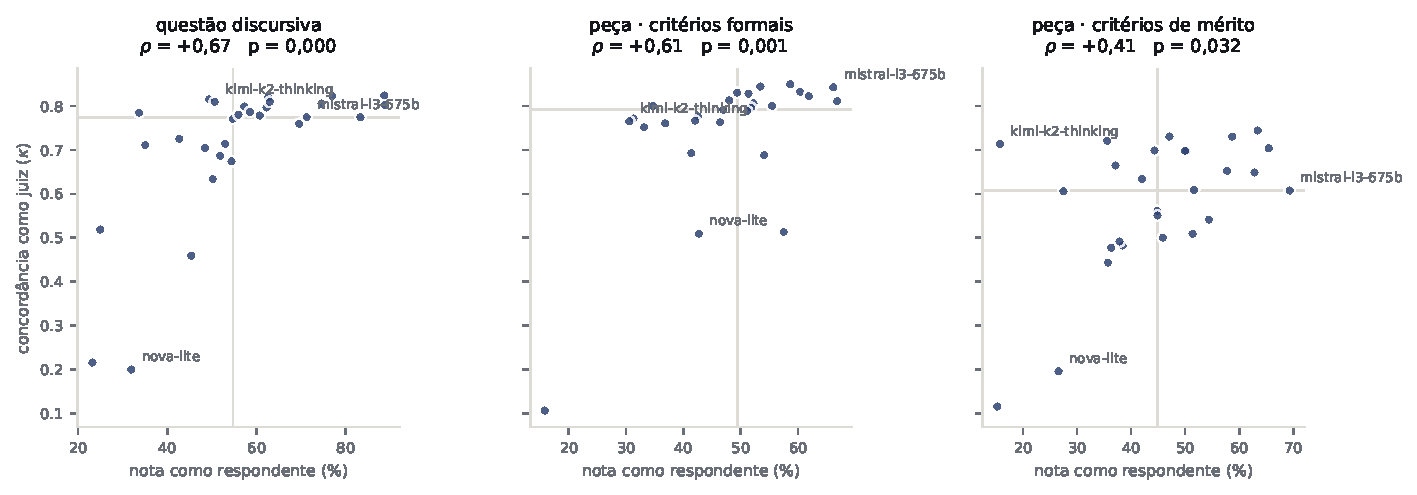
\includegraphics[width=\textwidth]{../artigo2/papeis}
\caption{Julgar contra responder, um painel por tarefa. Cada ponto é um modelo: nota como respondente no eixo horizontal, concordância como juiz no vertical. As linhas cinzas são as medianas. A associação enfraquece da esquerda para a direita, conforme a tarefa deixa de cobrar forma e passa a cobrar mérito.}
\end{figure}


A correlação de Spearman é de +0,67 na questão discursiva (n = 29, p = 0,0001), +0,61 nos critérios formais da peça (n = 27, p = 0,0008) e +0,41 nos de mérito (n = 27, p = 0,032). As três são positivas, e a ordem entre elas é o resultado: quanto mais a tarefa cobra julgamento de tese e menos cobra conformidade de formulário, menos o desempenho na tarefa prediz a competência de julgá-la. É o mesmo eixo que separa forma de mérito na Seção 4.3, agora visto do outro lado. O quadrante dos bons juízes que respondem mal está povoado nos três painéis, e os contraexemplos são fortes. O \texttt{kimi-k2-thinking} está entre os melhores juízes de peça e é o último colocado em escrever peça, com 15,8\% dos pontos de mérito. O \texttt{mistral-l3-675b} é o primeiro colocado em escrever peça e o décimo quarto como juiz. Sob seleção por desempenho na tarefa, os dois teriam sido classificados ao contrário. Se a associação em mérito é genuinamente mais fraca do que em discursiva é indecidível no nosso tamanho de amostra: o teste de Steiger para correlações dependentes [9] fica a 0,005 do corte convencional, e o intervalo de confiança da diferença por reamostragem vai de -0,18 a +0,55. A afirmação que se sustenta é que a associação existe, é positiva, e é fraca demais em mérito para substituir a calibração contra humanos.

\subsection{Combinar juízes, e o que as leituras por área sustentam}

Os vereditos gravados também respondem se combinar juízes supera o melhor juiz isolado. Dividimos as questões ao meio 200 vezes; em cada divisão os juízes são ordenados numa metade e a regra é medida na outra, de modo que escolha e medição nunca compartilham um item, e os resultados são a média das cinco repetições. O voto majoritário dos cinco melhores juízes eleva o $\kappa$ sobre o do melhor juiz isolado em 0,044 na questão discursiva, 0,038 nos critérios formais e 0,040 nos de mérito, e fica à frente em 91\%, 68\% e 86\% das divisões; os três melhores entregam cerca de três quartos desse ganho. Escolher o melhor juiz separadamente em cada área não ajuda: o $\kappa$ muda em +0,003, -0,017 e -0,026.

A razão é o tamanho das amostras por área. Um $\kappa$ por área se apoia em doze questões discursivas ou em três peças, e seu intervalo de 95\%, por bootstrap sobre as questões da área, tem largura mediana de 0,34 na questão discursiva, 0,41 nos critérios formais e 0,32 nos de mérito. A amplitude entre áreas dentro de um dos nove primeiros juízes, de 0,279 na mediana (Seção 4.1), é da mesma ordem. As tabelas por área descrevem, portanto, como cada juiz se saiu nestas questões; com esta amostra elas não estabelecem que um juiz seja melhor numa área do que em outra, e escolher o juiz por área é sobreajuste.

As divergências com o consenso humano também têm direção e lugar. Entre os nove melhores juízes de cada tarefa, a fração das divergências em que o juiz dá por cumprido um critério que os humanos não deram é de 30\% na questão discursiva, 36\% nos critérios formais e 59\% nos de mérito: no mérito, os juízes erram para o lado da leniência. E divergem menos nos critérios que pedem a citação de um dispositivo do que nos que pedem uma tese, 4,7\% contra 10,4\% dos critérios na questão discursiva e 7,5\% contra 15,0\% no mérito da peça. O código desta seção é \texttt{avaliacao/ensemble\_por\_area.py}, no repositório.

\section{Discussão}

As três medições apontam para a mesma coisa por caminhos independentes: competência jurídica de modelo de linguagem não é uma grandeza só, e a convenção de reportá-la como um número por modelo e por tarefa apaga justamente as diferenças que importam para quem vai usar o resultado. Escrever a peça correta e julgar se a peça alheia está correta são competências associadas a $\rho$ = 0,41 na parte que decide a nota. Acertar o endereçamento e acertar a tese são medidas que se ordenam de forma diferente e têm primeiros colocados diferentes. E o mesmo juiz, na mesma tarefa, concorda com o humano de forma muito distinta conforme a área do direito, com amplitude mediana de 0,279 dentro de um dos nove primeiros colocados, contra 0,047 de distância entre esses mesmos nove, ainda que, com doze questões ou três peças por área, essa amplitude esteja dentro da incerteza amostral (Seção 4.5).

A consequência prática mais direta é sobre a escolha de juiz. A pergunta "qual é o melhor juiz" está mal-posta antes de a resposta ser medida, porque a concordância agregada é uma média ponderada que reflete sobretudo a subtarefa mais numerosa: aqui, a classe de mérito tem 413 dos 561 critérios e determina 98\% da ordenação. A pergunta respondível é qual é o melhor juiz para a subtarefa que interessa e, havendo questões suficientes por área, para a área; e, onde nenhum juiz é claramente o melhor, a maioria dos melhores supera cada um deles (Seção 4.5). Quando existe uma decomposição externa disponível, e o espelho de correção de uma banca examinadora é uma decomposição pronta que o pesquisador não inventou, decompor antes de escolher custa pouco e muda a escolha.

A segunda consequência é sobre o que se pode publicar como ordem. Nos dados aqui, a ordem no topo não é informativa: nove juízes estão dentro do ruído uns dos outros em mérito de peça, e a ordem entre eles muda de execução para execução. O que propomos não é abandonar a tabela, e sim acompanhá-la do piso de ruído e marcar quais posições são distinguíveis. É barato: exige repetir o protocolo, o que os trabalhos cuidadosos já fazem, e converter a dispersão num limiar, o que quase ninguém faz. A reprodutibilidade tem pelo menos três camadas e a área reporta uma. A primeira é a amostragem: temperatura, número de amostras e semente, quando a API a aceita. A nossa não aceita, e medimos a dispersão resultante em vez de eliminá-la. A segunda é a configuração do servidor, tamanho de lote incluído, que no nosso teste à parte impediu que qualquer resposta se repetisse, embora esse teste não separe o lote da amostragem. A terceira é a identidade do modelo, e é a mais grave, porque nenhuma disciplina de código a resolve: o objeto medido está do outro lado de uma interface de programação, e o mesmo nome dois meses depois é outro modelo ou outra implementação, sem como saber qual. Um valor de $\kappa$ publicado é verificável dentro de uma janela de tempo e de uma configuração de inferência que ninguém descreve por inteiro.

\section{Limitações}

O padrão-ouro é de três anotadores e não foi ampliado: as 940 anotações são herdadas do Rabula [5], e o teto do experimento é o mesmo do original, a concordância entre os três anotadores, de 0,789 e 0,763. O benchmark tem 105 questões e sete áreas, o que é pouco para as leituras por área, em que cada célula repousa sobre 15 questões; a ampliação para 314 questões está planejada. O piso de ruído foi medido no melhor caso. O valor de 0,0101 mede apenas a variação sob amostragem repetida com o modelo de prompt fixo, e não inclui variação por mudança de prompt, de biblioteca ou de versão do modelo; o piso real entre laboratórios é necessariamente maior e não foi medido. Pelo mesmo motivo, a deriva de dois meses foi observada em um modelo e não medida sistematicamente. Todos os juízes receberam uma única formulação de prompt de julgamento, e é possível que alguns respondam melhor a outra e que a ordem mude com ela, o que não foi testado. A comparação entre as correlações dos três painéis da Figura 1 é limitada por poder amostral, como a própria Seção 4.4 declara. A redação de peça tem só três questões por área, de modo que as leituras por área desse gênero repousam sobre poucos casos. O agrupamento dos títulos de critério em forma e mérito é nosso e não foi validado por um anotador independente; o Apêndice D o lista por inteiro. Os dois juízes que corrigem os respondentes também estão entre os respondentes e corrigem as próprias respostas. Por fim, os cinco juízes Claude têm uma única amostra por repetição em vez de uma maioria de três, o que torna as suas repetições mais ruidosas que as dos demais.

\section{Conclusão}

Medimos 31 modelos de linguagem em três papéis sobre o mesmo material jurídico, as mesmas 105 questões da segunda fase do Exame de Ordem e os mesmos 940 critérios do espelho oficial, com padrão-ouro de 3 juristas, e reportamos os três papéis por área do direito e por classe de critério. Saber escrever uma peça e saber julgar a peça alheia são competências associadas, e a associação enfraquece conforme a tarefa deixa de cobrar forma e passa a cobrar mérito, de $\rho$ = 0,67 na questão discursiva a 0,41 nos critérios de mérito da peça. A redação de peça não é uma tarefa única para efeito de medição: separada nas classes que a banca rotula, ela produz duas ordens que concordam a $\rho$ = 0,48 e têm primeiros colocados diferentes. E a concordância de um mesmo juiz varia entre áreas do direito mais do que os juízes do topo variam entre si, mas, com esta amostra, essa variação está dentro da incerteza por área: a tabela por área descreve e ainda não serve para escolher; combinar os melhores juízes, ao contrário, compensa em todas as tarefas.

Daí saem três recomendações de reporte, e nenhuma exige dado novo. Reportar a tabela de concordância acompanhada do piso de ruído, marcando quais posições são distinguíveis, porque na nossa as nove primeiras não são. Decompor a tarefa antes de escolher o juiz sempre que exista uma decomposição externa disponível, porque a concordância agregada reflete a subtarefa mais numerosa e não necessariamente a que interessa. E reportar a configuração de amostragem e de servidor do juiz, temperatura, número de amostras, semente quando disponível e condições de lote, porque a saída depende de todas elas. Todas exigem apenas reportar o que já foi medido e é hoje descartado.

\appendix

\section{O prompt de julgamento}

O prompt é reproduzido abaixo como foi usado, na versão da questão discursiva; a versão da peça difere apenas na primeira frase, que descreve o exercício prático, e por omitir a frase sobre letras e partes da questão. Os campos entre chaves são preenchidos a cada chamada; \texttt{\{cache\_buster\}} é um comentário com um token hexadecimal aleatório, e o juiz deve devolver a soma dos dois inteiros aleatórios no campo \texttt{cache\_beaker} de cada veredito.

\begin{quote}\footnotesize\ttfamily\raggedright
Na segunda fase do exame da Ordem dos Advogados do Brasil o candidato deve responder a questões discursivas.\newline
~\newline
Você será o avaliador da resposta do candidato. Receberá 3 campos: 'gabarito', 'criterios' e 'resposta\_candidato'.\newline
O campo 'gabarito' é a referência oficial de resposta. O campo 'criterios' define os critérios objetivos para conferição de pontuação e o campo resposta\_candidato contém a resposta do candidato.\newline
~\newline
A persona que irá adotar para avaliar é uma examinador e professor de direito experiente com 10 anos de profissão.\newline
~\newline
Instruções de resposta:\newline
1. A resposta deve ser um json com o campo 'resultado' cujo conteúdo tem a mesma estrutura do JSON com os critérios mas com três campos a mais em cada linha: 'acerto', que pode ser 0 ou 1 a depender se o candidato satisfez o critério, 'raciocinio', que contém o motivo da decisão, resumidamente e 'cache\_beaker' contém a soma entre \{num1\} e \{num2\} .\newline
2. Os critérios de nota estão definidos no campo 'criterios'. Nele, há quanto cada cumprimento de critério confere de pontuação.\newline
3. O critério contém referências às letras da questão (A, B, C) e a parte dessa mesma questão, que funciona como um pedaço da questão.\newline
~\newline
REGRAS IMPORTANTES DE AVALIAÇÃO (cumpra todas):\newline
- Quando o critério contiver alternativas separadas por "ou" (ex.: "Art. X da CRFB/88 ou Súmula Vinculante n\textsuperscript{o} Y"), QUALQUER UMA das alternativas é suficiente para acerto=1. NÃO exija que o candidato cite todas.\newline
- Aceite paráfrases corretas e variações de redação do gabarito (ex.: "art. 71, III, da Constituição Federal" = "Art. 71, inciso III, da CRFB/88" = "artigo 71, III, CF").\newline
- Avalie o CONCEITO jurídico, não o match literal. Se o candidato expressou a ideia certa com outras palavras, é acerto=1.\newline
- Para critérios de citação legal: se o gabarito lista N referências como alternativas (com "ou"), basta o candidato citar 1 delas -- mesmo que com formato ligeiramente diferente -- para acerto=1.\newline
- Se o gabarito lista N elementos COM "e" (cumulativos), aí sim exija TODOS.\newline
~\newline
A resposta final não deve ter '''json porque isso quebra a lógica.\newline
~\newline
\{cache\_buster\}\newline
~\newline
RESPOSTA CANDIDATO\newline
´´´ \{resposta\_candidato\} ´´´\newline
~\newline
GABARITO\newline
´´´ \{gabarito\} ´´´\newline
~\newline
CRITERIOS\newline
´´´ \{criterios\} ´´´\newline
~\newline
JSON resposta:
\end{quote}

\section{Um item completo}

Direito administrativo, 41\textsuperscript{o} Exame, questão discursiva 1. O enunciado:

\begin{quote}\footnotesize\ttfamily\raggedright
Esglobênia, servidora pública federal estável, acreditava ter preenchido os respectivos requisitos do Regime Próprio de Previdência no cargo que ocupava, razão pela qual pleiteou e obteve, junto ao órgão de origem, a aposentadoria voluntária. Ato contínuo, o processo foi encaminhado ao Tribunal de Contas da União, o qual verificou algumas inconsistências no deferimento do pedido, de modo que está tendente a negar o registro da aposentadoria, sendo certo que o processo chegou na Corte de Contas há apenas um ano. Diante dessa situação hipotética, responda como advogado(a), fundamentadamente, aos questionamentos a seguir. A) O ato aposentadoria de Esglobênia estava perfeito, ou seja, completou o seu ciclo de formação, antes do pronunciamento da Corte de Contas? Justifique. (Valor: 0,60) B) Para negar o registro da aposentadoria de Esglobênia, o Tribunal de Contas precisa observar a ampla defesa e o contraditório? Justifique. (Valor: 0,65) Obs.: o(a) examinando(a) deve fundamentar as respostas. A mera citação do dispositivo legal não confere pontuação.
\end{quote}

A resposta avaliada, escrita pelo GPT-4o mini, como os anotadores humanos e os juízes a viram:

\begin{quote}\footnotesize\ttfamily\raggedright
A) O ato de aposentadoria de Esglobênia não estava perfeito, pois o processo de aposentadoria ainda estava sujeito à análise do Tribunal de Contas da União (TCU), que possui a competência para apreciar a legalidade dos atos administrativos, incluindo a aposentadoria de servidores públicos. O ciclo de formação do ato se completa com o registro pelo TCU, e enquanto este não ocorrer, o ato permanece sob análise e pode ser considerado irregular.\newline
~\newline
B) Sim, para negar o registro da aposentadoria de Esglobênia, o Tribunal de Contas deve observar o princípio da ampla defesa e do contraditório. Isso se deve ao fato de que a negativa de registro implica em uma decisão que pode afetar diretamente os direitos da servidora, sendo necessário garantir que ela tenha a oportunidade de se manifestar e apresentar suas razões antes que uma decisão desfavorável seja tomada.
\end{quote}

Os quatro critérios da banca:

\begin{itemize}
\item \textbf{A-I} (0,50 pontos). Não. A concessão de aposentadoria configura ato complexo que só estará perfeito após pronunciamento da Corte de Contas
\item \textbf{A-II} (0,10 pontos). nos termos do Art. 71, inciso III, da CRFB/88 ou Súmula Vinculante n\textsuperscript{o} 3
\item \textbf{B-I} (0,55 pontos). Não. O contraditório e a ampla defesa são assegurados no Tribunal de Contas da União quando da decisão puder resultar anulação ou revogação de ato administrativo, excetuada a apreciação de legalidade do ato de concessão inicial de aposentadoria, reforma e pensão
\item \textbf{B-II} (0,10 pontos). consoante a Súmula Vinculante n\textsuperscript{o} 3
\end{itemize}

A Tabela 6 traz, para cada critério, o veredito de cada anotador e o do Kimi K2.5 em cada uma das cinco repetições, como maioria de três amostras. Nas repetições 1 e 2, uma das três amostras marcou o critério A-I como não cumprido; a maioria recupera o veredito, e é essa a variação que o piso de ruído da Seção 4.2 mede.

\begin{table}[!ht]
\centering
\caption{O item do Apêndice B: critérios, pontuação, os três vereditos humanos e o veredito por maioria do Kimi K2.5 em cada uma das cinco repetições (1 = cumprido).}
\footnotesize\setlength{\tabcolsep}{2pt}
\begin{tabular}{llrr}
\hline
\textbf{Critério} & \textbf{Pontos} & \textbf{Humanos} & \textbf{Kimi, rep. 1--5} \\
\hline
A-I & 0,50 & 1 / 1 / 1 & 1 1 1 1 1 \\
A-II & 0,10 & 0 / 0 / 0 & 0 0 0 0 0 \\
B-I & 0,55 & 0 / 0 / 0 & 0 0 0 0 0 \\
B-II & 0,10 & 0 / 0 / 0 & 0 0 0 0 0 \\
\hline
\end{tabular}
\end{table}


\section{Configuração dos juízes}

Os 31 juízes rodam a temperatura 0,2, sem semente, com o prompt do Apêndice A. O teto de saída é o solicitado; quando a resposta é cortada, ele é dobrado até 32.000 tokens ou até o limite que o modelo aceita. Amostras é o número de chamadas independentes por questão em cada repetição, combinadas por voto de maioria. Os respondentes rodam a temperatura 0,7, com teto de saída de 2.500 tokens e três execuções por questão.

\begin{table}[!ht]
\centering
\caption{Os juízes: API do provedor, identificador do modelo, teto de saída solicitado em tokens e amostras por repetição.}
\footnotesize\setlength{\tabcolsep}{2pt}
\begin{tabular}{llrrr}
\hline
\textbf{Juiz} & \textbf{API} & \textbf{Identificador do modelo} & \textbf{Teto} & \textbf{Amostras} \\
\hline
claude-haiku-4-5 & Bedrock & \texttt{us.anthropic.claude-haiku-4-5-20251001-v1:0} & 8.000 & 1 \\
claude-opus-4-5 & Bedrock & \texttt{us.anthropic.claude-opus-4-5-20251101-v1:0} & 8.000 & 1 \\
claude-opus-4-6 & Bedrock & \texttt{us.anthropic.claude-opus-4-6-v1} & 8.000 & 1 \\
claude-sonnet-4-5 & Bedrock & \texttt{us.anthropic.claude-sonnet-4-5-20250929-v1:0} & 8.000 & 1 \\
claude-sonnet-4-6 & Bedrock & \texttt{us.anthropic.claude-sonnet-4-6} & 8.000 & 1 \\
deepseek-v3 & Bedrock & \texttt{deepseek.v3.2} & 8.000 & 3 \\
glm-4-7 & Bedrock & \texttt{zai.glm-4.7} & 8.000 & 3 \\
glm-5 & Bedrock & \texttt{zai.glm-5} & 8.000 & 3 \\
gpt-oss-120b & Bedrock & \texttt{openai.gpt-oss-120b-1:0} & 16.000 & 3 \\
kimi-k2-5 & Bedrock & \texttt{moonshotai.kimi-k2.5} & 16.000 & 3 \\
kimi-k2-thinking & Bedrock & \texttt{moonshot.kimi-k2-thinking} & 16.000 & 3 \\
llama3-3-70b & Bedrock & \texttt{us.meta.llama3-3-70b-instruct-v1:0} & 2.048 & 3 \\
llama3-70b & Bedrock & \texttt{meta.llama3-70b-instruct-v1:0} & 2.048 & 3 \\
llama3-8b & Bedrock & \texttt{meta.llama3-8b-instruct-v1:0} & 2.048 & 3 \\
llama4-maverick & Bedrock & \texttt{us.meta.llama4-maverick-17b-instruct-v1:0} & 8.000 & 3 \\
llama4-scout & Bedrock & \texttt{us.meta.llama4-scout-17b-instruct-v1:0} & 8.000 & 3 \\
magistral-small & Bedrock & \texttt{mistral.magistral-small-2509} & 16.000 & 3 \\
minimax-m2-5 & Bedrock & \texttt{minimax.minimax-m2.5} & 8.000 & 3 \\
mistral-l3-675b & Bedrock & \texttt{mistral.mistral-large-3-675b-instruct} & 8.000 & 3 \\
mistral-large & Bedrock & \texttt{mistral.mistral-large-2402-v1:0} & 8.000 & 3 \\
mistral-small & Bedrock & \texttt{mistral.mistral-small-2402-v1:0} & 2.048 & 3 \\
mixtral-8x7b & Bedrock & \texttt{mistral.mixtral-8x7b-instruct-v0:1} & 4.096 & 3 \\
nemotron-s3-120b & Bedrock & \texttt{nvidia.nemotron-super-3-120b} & 8.000 & 3 \\
nova-lite & Bedrock & \texttt{amazon.nova-lite-v1:0} & 8.000 & 3 \\
nova-micro & Bedrock & \texttt{amazon.nova-micro-v1:0} & 8.000 & 3 \\
nova-pro & Bedrock & \texttt{amazon.nova-pro-v1:0} & 8.000 & 3 \\
qwen3-235b-vl & Bedrock & \texttt{qwen.qwen3-vl-235b-a22b} & 8.000 & 3 \\
qwen3-32b & Bedrock & \texttt{qwen.qwen3-32b-v1:0} & 8.000 & 3 \\
qwen3-80b-a3b & Bedrock & \texttt{qwen.qwen3-next-80b-a3b} & 8.000 & 3 \\
sabia-4 & Maritaca & \texttt{sabia-4} & 8.000 & 3 \\
sabiazinho-4 & Maritaca & \texttt{sabiazinho-4} & 8.000 & 3 \\
\hline
\end{tabular}
\end{table}


\section{Títulos de critério por classe}

A banca dá um título a cada critério da peça. Agrupamos os 60 títulos distintos nas duas classes da Seção 3.2; o número de critérios com cada título está entre parênteses. Nenhum título cai nas duas classes.

\textbf{Forma} (148 critérios): Endereçamento (56); Fechamento (22); Partes e Fundamento Legal (10); Qualificação das partes (9); Prazo e Fechamento (6); Gratuidade de justiça e prioridade (4); Interposição (4); Petição de Interposição (4); Requisitos de admissibilidade recursal (4); Tempestividade (4); ENDEREÇAMENTO (3); Procedimento (3); Requisitos de Admissibilidade Recursal (3); Encerramento (2); Honorários advocatícios (2); Partes (2); Peça (2); Qualificação dos interessados/ requerentes (2); Requisitos Tempestividade (2); Valor da causa / Fechamento (2); FECHAMENTO (1); Menção ao valor da causa (1).

\textbf{Mérito} (413 critérios): Pedidos (71); Fundamentação (55); Fundamentos de mérito (34); Fundamentação Jurídica/Legal (23); Razões recursais (21); Mérito (20); Razões de apelação (19); Cabimento (14); Direitos lesados (14); Fatos e Alegações de Mérito (12); Fundamentos jurídicos (12); Requerimentos (11); Legitimidade (9); PEDIDOS (9); Direitos violados (8); Fundamentos (8); Vínculo e verbas pela extinção (7); Das Provas (6); Fundamentos da cautelar (6); DAS PROVAS E DO DEMONSTRATIVO DO DÉBITO ATUALIZADO (5); Dano Patrimonial (material) (5); Dos Pedidos (5); Fundamentos da liminar (5); Alegações Preliminares (4); Cabimento da ADC (4); FUNDAMENTOS JURÍDICOS (3); Prova domínio e qualidade de terceiro (3); Tutela provisória de urgência (3); DO TÍTULO EXECUTIVO EXTRAJUDICIAL (2); Dano Extrapatrimonial (2); Do litisconsórcio unitário (2); Fundamentos para a concessão da medida liminar (2); LEGITIMIDADE ATIVA (2); LEGITIMIDADE PASSIVA (2); Pedido (2); Fatos (1); Legitimidade ativa (1); Razões (1).

\section*{Agradecimentos e declarações}

\textbf{Uso de IA generativa.} Modelos generativos são o objeto de estudo deste trabalho, nos três papéis descritos na Seção 3.3, e todos os números reportados vêm da execução do código depositado sobre os julgamentos depositados. Além disso, os autores usaram um modelo de linguagem para auxiliar na escrita do código de análise e de montagem do manuscrito, e na redação do texto, composto primeiro em português. Nenhum número foi transcrito a mão, e cada referência foi conferida contra a fonte primária. Os autores revisaram e editaram todo o conteúdo e assumem responsabilidade integral por ele.

\begin{thebibliography}{99}
\bibitem{r1} Zheng, L., Chiang, W.-L., Sheng, Y., Zhuang, S., Wu, Z., Zhuang, Y., Lin, Z., Li, Z., Li, D., Xing, E. P., Zhang, H., Gonzalez, J. E., Stoica, I. \emph{Judging LLM-as-a-Judge with MT-Bench and Chatbot Arena}. NeurIPS, 2023.
\bibitem{r2} Guha, N. et al. \emph{LegalBench: A Collaboratively Built Benchmark for Measuring Legal Reasoning in Large Language Models}. NeurIPS Datasets and Benchmarks, 2023.
\bibitem{r3} Pires, R., Malaquias Junior, R., Nogueira, R. \emph{Automatic Legal Writing Evaluation of LLMs}. ICAIL '25: Proceedings of the Twentieth International Conference on Artificial Intelligence and Law, 420--424, 2025. doi:10.1145/3769126.3769227.
\bibitem{r4} Pires, R., Sales Almeida, T., Larcher Junior, C., Bonás, G., Abonizio, H., Piau, M., Malaquias Junior, R., Laitz, T., Nogueira, R. \emph{Magis-Bench: Evaluating LLMs on Magistrate-Level Legal Tasks}. arXiv:2605.08437, 2026.
\bibitem{r5} Pacheco, E. C. B., Suriani, F. M., Ribeiro, R. \emph{Rabula: A Benchmark for Evaluating LLMs in Brazilian Legal Tasks}. Proceedings of the First Argument Mining and Empirical Legal Research Workshop (AMELR 2025), CEUR-WS Vol-4089, paper 6, 2025.
\bibitem{r6} Goldberg, D. \emph{What Every Computer Scientist Should Know About Floating-Point Arithmetic}. ACM Computing Surveys, 23(1), 5--48, 1991.
\bibitem{r7} Cohen, J. \emph{A Coefficient of Agreement for Nominal Scales}. Educational and Psychological Measurement, 20(1), 37--46, 1960.
\bibitem{r8} Fleiss, J. L. \emph{Measuring Nominal Scale Agreement Among Many Raters}. Psychological Bulletin, 76(5), 378--382, 1971.
\bibitem{r9} Steiger, J. H. \emph{Tests for Comparing Elements of a Correlation Matrix}. Psychological Bulletin, 87(2), 245--251, 1980.
\bibitem{r10} Pacheco, E., Russo, C. M. \emph{Corpus sintético na adaptação de modelos de linguagem ao direito brasileiro}. Artigo companheiro, em preparação, 2026.
\bibitem{r11} Pacheco, E., Russo, C. M. \emph{Agreement of 31 candidate automatic judges against a human gold standard on Brazilian legal tasks}, v1.0 [Conjunto de dados]. Zenodo, 2026. doi:10.5281/zenodo.22739161.
\bibitem{r12} Pacheco, E., Russo, C. M. \emph{Paired raw and structured corpora for Brazilian legal domain adaptation}, v1.0 [Conjunto de dados]. Zenodo, 2026. doi:10.5281/zenodo.22739216.
\bibitem{r13} Pacheco, E., Russo, C. M. \emph{Judgments of 180 trained conditions on a Brazilian Bar Examination benchmark}, v1.0 [Conjunto de dados]. Zenodo, 2026. doi:10.5281/zenodo.22739184.
\bibitem{r14} Pacheco, E. \emph{Medindo a competência de LLMs no direito brasileiro: responder, redigir e julgar} [Código-fonte]. github.com/eduardocbpacheco/measuring-llm-competence-brazilian-law-, 2026.
\bibitem{r15} Thakur, A. S., Choudhary, K., Ramayapally, V. S., Vaidyanathan, S., Hupkes, D. \emph{Judging the Judges: Evaluating Alignment and Vulnerabilities in LLMs-as-Judges}. Proceedings of the Fourth Workshop on Generation, Evaluation and Metrics (GEM\textsuperscript{2}), 2025. arXiv:2406.12624.
\bibitem{r16} Tan, S., Zhuang, S., Montgomery, K., Tang, W. Y., Cuadron, A., Wang, C., Popa, R. A., Stoica, I. \emph{JudgeBench: A Benchmark for Evaluating LLM-based Judges}. ICLR, 2025.
\bibitem{r17} Zeng, Z., Yu, J., Gao, T., Meng, Y., Goyal, T., Chen, D. \emph{Evaluating Large Language Models at Evaluating Instruction Following}. ICLR, 2024.
\bibitem{r18} Panickssery, A., Bowman, S. R., Feng, S. \emph{LLM Evaluators Recognize and Favor Their Own Generations}. NeurIPS, 2024.
\bibitem{r19} Feinstein, A. R., Cicchetti, D. V. \emph{High Agreement but Low Kappa: I. The Problems of Two Paradoxes}. Journal of Clinical Epidemiology, 43(6), 543--549, 1990.
\bibitem{r20} Byrt, T., Bishop, J., Carlin, J. B. \emph{Bias, Prevalence and Kappa}. Journal of Clinical Epidemiology, 46(5), 423--429, 1993.
\bibitem{r21} Gwet, K. L. \emph{Computing Inter-Rater Reliability and Its Variance in the Presence of High Agreement}. British Journal of Mathematical and Statistical Psychology, 61(1), 29--48, 2008.
\end{thebibliography}
\end{document}
